%File: anonymous-submission-latex-2023.tex
\documentclass[letterpaper]{article} % DO NOT CHANGE THIS
\usepackage[submission]{aaai23}  % DO NOT CHANGE THIS
\usepackage{times}  % DO NOT CHANGE THIS
\usepackage{helvet}  % DO NOT CHANGE THIS
\usepackage{courier}  % DO NOT CHANGE THIS
\usepackage[hyphens]{url}  % DO NOT CHANGE THIS
\usepackage{graphicx} % DO NOT CHANGE THIS
\urlstyle{rm} % DO NOT CHANGE THIS
\def\UrlFont{\rm}  % DO NOT CHANGE THIS
\usepackage{natbib}  % DO NOT CHANGE THIS AND DO NOT ADD ANY OPTIONS TO IT
\usepackage{caption} % DO NOT CHANGE THIS AND DO NOT ADD ANY OPTIONS TO IT
\frenchspacing  % DO NOT CHANGE THIS
\setlength{\pdfpagewidth}{8.5in} % DO NOT CHANGE THIS
\setlength{\pdfpageheight}{11in} % DO NOT CHANGE THIS

\usepackage{mathtools}
\usepackage{amsthm}
\usepackage{amssymb}
\usepackage{pifont}
\usepackage[linesnumbered,ruled,vlined]{algorithm2e}
\usepackage{tikz}
\usepackage[capitalize]{cleveref}
\usepackage{booktabs}
\usepackage{multirow}
\usepackage{colortbl}
\usepackage{complexity}

% These are recommended to typeset algorithms but not required. See the subsubsection on algorithms. Remove them if you don't have algorithms in your paper.
% \usepackage{algorithm}
% \usepackage{algorithmic}

% These are recommended to typeset listings but not required. See the subsubsection on listing. Remove this block if you don't have listings in your paper.
% \usepackage{newfloat}
% \usepackage{listings}
% \DeclareCaptionStyle{ruled}{labelfont=normalfont,labelsep=colon,strut=off} % DO NOT CHANGE THIS
% \lstset{%
% 	basicstyle={\footnotesize\ttfamily},% footnotesize acceptable for monospace
% 	numbers=left,numberstyle=\footnotesize,xleftmargin=2em,% show line numbers, remove this entire line if you don't want the numbers.
% 	aboveskip=0pt,belowskip=0pt,%
% 	showstringspaces=false,tabsize=2,breaklines=true}
% \floatstyle{ruled}
% \newfloat{listing}{tb}{lst}{}
% \floatname{listing}{Listing}

% Keep the \pdfinfo as shown here. There's no need
% for you to add the /Title and /Author tags.
\pdfinfo{
/TemplateVersion (2023.1)
}

% DISALLOWED PACKAGES
% \usepackage{authblk} -- This package is specifically forbidden
% \usepackage{balance} -- This package is specifically forbidden
% \usepackage{color (if used in text)
% \usepackage{CJK} -- This package is specifically forbidden
% \usepackage{float} -- This package is specifically forbidden
% \usepackage{flushend} -- This package is specifically forbidden
% \usepackage{fontenc} -- This package is specifically forbidden
% \usepackage{fullpage} -- This package is specifically forbidden
% \usepackage{geometry} -- This package is specifically forbidden
% \usepackage{grffile} -- This package is specifically forbidden
% \usepackage{hyperref} -- This package is specifically forbidden
% \usepackage{navigator} -- This package is specifically forbidden
% (or any other package that embeds links such as navigator or hyperref)
% \indentfirst} -- This package is specifically forbidden
% \layout} -- This package is specifically forbidden
% \multicol} -- This package is specifically forbidden
% \nameref} -- This package is specifically forbidden
% \usepackage{savetrees} -- This package is specifically forbidden
% \usepackage{setspace} -- This package is specifically forbidden
% \usepackage{stfloats} -- This package is specifically forbidden
% \usepackage{tabu} -- This package is specifically forbidden
% \usepackage{titlesec} -- This package is specifically forbidden
% \usepackage{tocbibind} -- This package is specifically forbidden
% \usepackage{ulem} -- This package is specifically forbidden
% \usepackage{wrapfig} -- This package is specifically forbidden
% DISALLOWED COMMANDS
% \nocopyright -- Your paper will not be published if you use this command
% \addtolength -- This command may not be used
% \balance -- This command may not be used
% \baselinestretch -- Your paper will not be published if you use this command
% \clearpage -- No page breaks of any kind may be used for the final version of your paper
% \columnsep -- This command may not be used
% \newpage -- No page breaks of any kind may be used for the final version of your paper
% \pagebreak -- No page breaks of any kind may be used for the final version of your paperr
% \pagestyle -- This command may not be used
% \tiny -- This is not an acceptable font size.
% \vspace{- -- No negative value may be used in proximity of a caption, figure, table, section, subsection, subsubsection, or reference
% \vskip{- -- No negative value may be used to alter spacing above or below a caption, figure, table, section, subsection, subsubsection, or reference

\setcounter{secnumdepth}{2} %May be changed to 1 or 2 if section numbers are desired.

% Title

% Your title must be in mixed case, not sentence case.
% That means all verbs (including short verbs like be, is, using,and go),
% nouns, adverbs, adjectives should be capitalized, including both words in hyphenated terms, while
% articles, conjunctions, and prepositions are lower case unless they
% directly follow a colon or long dash
\title{Recursive Solutions to First-Order Model Counting}
\author{Anonymous Submission}
\affiliations{}

\usetikzlibrary{cd}
\usetikzlibrary{shapes}

\crefname{algocf}{algorithm}{Algorithms}
\Crefname{algocf}{Algorithm}{Algorithms}

\newcommand{\crefrangeconjunction}{--}
\newcommand\pfun{\mathrel{\ooalign{\hfil$\mapstochar\mkern5mu$\hfil\cr$\to$\cr}}}
\newcommand{\cmark}{\ding{51}}%
\newcommand{\xmark}{\ding{55}}%
\newcommand{\FOtwo}{$\mathsf{FO}^{2}$}
\newcommand{\FOthree}{$\mathsf{FO}^{3}$}
\newcommand{\SFO}{$\mathsf{S}^{2}\mathsf{FO}^{2}$}
\newcommand{\SRU}{$\mathsf{S}^{2}\mathsf{RU}$}
\newcommand{\Uone}{$\mathsf{U}_{1}$}
\newcommand{\Ctwo}{$\mathsf{C}^{2}$}
\newcommand{\IFO}{$\mathsf{I}\mathsf{FO}^{2}$}
\DeclareMathOperator{\CR}{\textsc{CR}}
\DeclareMathOperator{\GDR}{\textsc{GDR}}
\DeclareMathOperator{\Reff}{\textsc{Ref}}
\DeclareMathOperator{\dom}{dom}
\DeclareMathOperator{\Doms}{Doms}
\DeclareMathOperator{\Vars}{Vars}
\SetKwProg{Fn}{Function}{:}{}
\SetKwFunction{identifyRecursion}{r}
\SetKwFunction{generateMaps}{genMaps}
\newtheorem{conjecture}{Conjecture}
\theoremstyle{definition}
\newtheorem{definition}{Definition}
\newtheorem{example}{Example}
\makeatletter
\newcommand{\nosemic}{\renewcommand{\@endalgocfline}{\relax}}% Drop semi-colon ;
\newcommand{\dosemic}{\renewcommand{\@endalgocfline}{\algocf@endline}}% Reinstate semi-colon ;
\newcommand{\pushline}{\Indp}% Indent
\newcommand{\popline}{\Indm\dosemic}% Undent
\makeatother
\Crefname{algocf}{Algorithm}{Algorithms}
\crefname{line}{line}{lines}

\begin{document}

\maketitle

\begin{abstract}
  First-order model counting (FOMC) is a computational problem that asks to
  count the models of a sentence in finite-domain first-order logic. Despite
  being around for more than a decade, practical FOMC algorithms are still
  unable to compute functions as simple as a factorial. We argue that the
  capabilities of FOMC algorithms to date are limited by their inability to
  express arbitrary recursive computations. To enable arbitrary recursion, we
  relax the restrictions that typically accompany domain recursion and
  generalise circuits used to express a solution to an FOMC problem to graphs
  that may contain cycles. To this end, we enhance the most well-established
  (weighted) FOMC algorithm \textsc{ForcLift} with new compilation rules and an
  algorithm to check whether a recursive call is feasible. These improvements
  allow the algorithm to construct efficient solutions to counting fundamental
  structures such as injections and bijections. We end with a few conjectures on
  what classes of instances could be liftable as a result.
\end{abstract}

\section{Introduction}

% 1. What is the problem?
% 2. Why is it interesting and important?

\emph{First-order model counting} (FOMC) is the problem of computing the number
of models of a sentence in first-order logic (FOL) given the size(s) of its
domain(s) \citep{DBLP:conf/pods/BeameBGS15}. \emph{Symmetric weighted FOMC}
(WFOMC) extends FOMC with (pairs of) weights on predicates and asks for a
weighted sum across all models instead. By fixing the sizes of the domains, a
WFOMC instance can be rewritten as an instance of (propositional) weighted model
counting \citep{DBLP:journals/ai/ChaviraD08}. WFOMC emerged as the dominant
approach to \emph{lifted (probabilistic) inference}. Lifted inference techniques
exploit symmetries in probabilistic models by reasoning about sets rather than
individuals \citep{DBLP:conf/ecai/Kersting12}. By doing so, many instances
become solvable in polynomial time \citep{DBLP:conf/nips/Broeck11}. Lifted
inference algorithms are typically used on probabilistic models such as
probabilistic programming languages
\citep{DBLP:journals/ml/RaedtK15,DBLP:journals/ijar/RiguzziBZCL17}, Markov logic
networks
\citep{DBLP:conf/ijcai/BroeckTMDR11,DBLP:journals/cacm/GogateD16,DBLP:journals/ml/RichardsonD06},
and other lifted graphical \citep{DBLP:journals/ml/KimmigMG15} and statistical
relational \citep{DBLP:series/synthesis/2016Raedt} models. Lifted inference
techniques for probabilistic databases, while developed somewhat independently,
have also been inspired by WFOMC
\citep{DBLP:journals/pvldb/GatterbauerS15,DBLP:journals/debu/GribkoffSB14}.
While WFOMC tends to receive more attention in the literature, FOMC is an
interesting problem in an of itself because of its connections to finite model
theory \citep{DBLP:conf/kr/BremenK21} and applications in enumerative
combinatorics \citep{DBLP:conf/ilp/BarvinekB0ZK21}.

% 3. Why is it hard? (E.g., why do naive approaches fail?)
% complexity/liftability -> murky boundary

Traditionally in computational complexity theory, a problem is \emph{tractable}
if it can be solved in time polynomial in the instance size. The equivalent
notion in (W)FOMC is liftability. A (W)FOMC instance is \emph{(domain-)liftable}
if it can be solved in time polynomial in the size(s) of the domain(s)
\citep{jaeger2012liftability}. Over more than a decade, many classes of
instances were shown to be liftable
\citep{DBLP:conf/kr/BremenK21,DBLP:conf/nips/KazemiKBP16,DBLP:conf/lics/KuusistoL18,DBLP:journals/jair/Kuzelka21}.
First, \citet{DBLP:conf/nips/Broeck11} showed that the class of all sentences of
FOL with up to two variables (denoted \FOtwo{}) is liftable. Then
\citet{DBLP:conf/pods/BeameBGS15} proved that there exists a sentence with three
variables for which FOMC is $\#\P_{1}$-complete (i.e., \FOthree{} is not
liftable). Since these two results came out, most of the research on (W)FOMC
focused on developing faster solutions for the \FOtwo{} fragment
\citep{DBLP:conf/uai/BremenK21,DBLP:conf/aaai/MalhotraS22} and defining new
liftable fragments. These fragments include \SFO{} and \SRU{}
\citep{DBLP:conf/nips/KazemiKBP16}, \Uone{} \citep{DBLP:conf/lics/KuusistoL18},
\FOtwo{} with tree axioms \citep{DBLP:conf/kr/BremenK21}, and \Ctwo{} (i.e., the
two-variable fragment with counting quantifiers)
\citep{DBLP:journals/jair/Kuzelka21,DBLP:conf/aaai/MalhotraS22}. On the
empirical front, there are several open-source implementations of exact WFOMC
algorithms: \textsc{ForcLift} \citep{DBLP:conf/ijcai/BroeckTMDR11},
probabilistic theorem proving \citep{DBLP:journals/cacm/GogateD16}, and
\textsc{L2C} \citep{DBLP:conf/kr/KazemiP16}. Approximate counting is supported
by \textsc{ApproxWFOMC} \citep{DBLP:conf/ijcai/BremenK20} as well as
\textsc{ForcLift} \citep{DBLP:conf/uai/BroeckCD12} and probabilistic theorem
proving \citep{DBLP:journals/cacm/GogateD16}.

% 4. Why hasn't it been solved before? (Or, what's wrong with previous proposed
% solutions? How does mine differ?)
% simple unliftable instances -> recursion

However, none of the publicly available exact (W)FOMC algorithms can efficiently
compute functions as simple as a factorial.\footnote{The problem of computing
  the factorial can be described using two variables and counting quantifiers,
  so it is known to be liftable in principle
  \citep{DBLP:journals/jair/Kuzelka21}, but an algorithm that can lift such an
  instance in practice does not exist.} We claim that this shortcoming is due to
the inability of these algorithms to construct recursive solutions. The topic of
recursion in the context of WFOMC has been studied before but in limited ways.
\Citet{DBLP:conf/ilp/BarvinekB0ZK21} use WFOMC to generate numerical data that
is then used to conjecture recurrence relations that explain that data.
\Citet{DBLP:conf/nips/Broeck11} introduced the idea of \emph{domain recursion}.
Intuitively, domain recursion partitions a domain of size $n$ into a single
explicitly named constant and the remaining domain of size $n-1$. However, many
stringent conditions are enforced to ensure that the search for a tractable
solution always terminates.

% 5. What are the key components of my approach and results? Also include any
% specific limitations.

% 5.1) An overview of how ForcLift/Crane work.

In this work, we show how to relax these restrictions in a way that results in a
stronger (W)FOMC algorithm, capable of handling more instances (e.g., counting
various injective mappings) in a lifted manner. The ideas presented in this
paper are implemented in \textsc{Crane}---an extension of the arguably most
well-known WFOMC algorithm \textsc{ForcLift}. \textsc{ForcLift} works in two
stages: compilation and evaluation/propagation. In the first stage, various
\emph{(compilation) rules} are applied to the input (or some derivative)
formula, gradually constructing a circuit. In the second stage, the weights of
the instance are propagated through the circuit, computing the weighted model
count. Along with new compilation rules, \textsc{Crane} introduces changes to
both stages of the process. First, while \textsc{ForcLift} applies compilation
rules via greedy\footnote{The algorithm is not described in any paper but can be
  found in its source code at \url{https://dtai.cs.kuleuven.be/drupal/wfomc}}
search, \textsc{Crane} uses a hybrid search algorithm that applies some rules
greedily and some using breadth-first search. Second, the product of compilation
is not directly evaluated but rather interpreted as a collection of functions on
domain sizes.

% \footnote{There is also an intermediate stage called \emph{smoothing} that takes
%   place between compilation and evaluation. As our changes to smoothing are
%   rather elementary, we do not discuss them to not distract the reader from the
%   main contributions of this paper.}

% 5.2) The main idea: cycles that represent recursive calls.

The main conceptual difference between \textsc{Crane} and \textsc{ForcLift} is
that we utilise labelled directed graphs instead of circuits, where cycles
represent recursive calls. Suppose the input formula $\phi$ depends on a domain
of size $n \in \mathbb{N}$. \emph{Generalised domain recursion} (GDR)---one of
the new compilation rules---transforms $\phi$ into a different formula $\psi$
that has an additional constant and some new \emph{constraints}. After some
additional transformations, the constraints in $\psi$ become `uniform' and can
be removed, replacing the domain of size $n$ with a new domain of size
$n-1$---this is the responsibility of the \emph{constraint removal} (CR)
compilation rule. Afterwards, another compilation rule recognizes that the
resulting formula is just like the input formula $\phi$ but with a different
domain. This observation allows us to add a cycle-forming edge to the graph,
which can be interpreted as function $f$ relying on $f(n-1)$ to compute $f(n)$.

% search
% interpretation

% 5.3) contributions, references to sections, shortcomings

We begin by defining the representation used for sentences in FOL in
\cref{sec:recprelims}. Then, in \cref{sec:methods}, we define the graphs that
replace circuits in representing a solution to a (W)FOMC problem.
\Cref{sec:rules} introduces the new compilation rules. In \cref{sec:interpret},
we discuss how a graph can be interpreted as a collection of (potentially
recursive) functions. In \cref{sec:results}, we compare \textsc{ForcLift} and
\textsc{Crane} on a range of function-counting problems. We show that
\textsc{Crane} performs as well as \textsc{ForcLift} on the instances that were
already solvable by \textsc{ForcLift} but is also able to handle most of the
instances that \textsc{ForcLift} fails on. Finally, in \cref{sec:conclusion}, we
conclude by outlining some conjectures and directions for future work.

\section{Preliminaries}\label{sec:recprelims}

Our representation of FOMC instances is largely based on the format used
internally by \textsc{ForcLift}, some aspects of which are described by
\citet{DBLP:conf/ijcai/BroeckTMDR11}. \textsc{ForcLift} can translate sentences
in a variant of function-free many-sorted FOL with equality to this internal
format. We use lowercase Latin letters for predicates and constants, uppercase
Latin letters for variables, and uppercase Greek letters for domains. An
\emph{atom} is $p(t_1, \dots, t_n)$ for some predicate $p$ and terms
$t_{1}, \dots, t_{n}$. A \emph{term} is either a constant or a variable. A
\emph{literal} is either an atom or the negation of an atom (denoted by
$\neg p(t_1, \dots, t_n)$). Let $\mathcal{D}$ be the set of all (finite)
domains. Initially, $\mathcal{D}$ contains all domains mentioned by the input
(W)FOMC instance. During compilation, new domains are added to $\mathcal{D}$ by
some of the compilation rules. Each such new domain is interpreted as a subset
of some element of $\mathcal{D}$.

\begin{definition}[Constraint]\label{def:constraint}
  An \emph{(inequality) constraint} is a pair $(a, b)$, where $a$ is a variable,
  and $b$ is either a variable or a constant.
\end{definition}

\begin{definition}[Clause]\label{def:clause}
  A \emph{clause}\footnote{\citet{DBLP:conf/ijcai/BroeckTMDR11} refer to clauses
    as c-clauses.} is a triple $c = (L, C, \delta_c)$, where $L$ is a set of
  literals, $C$ is a set of constraints, and $\delta_c$ is the domain map of
  $c$. Let $\Vars$ be the function that maps clauses and sets of either literals
  or constraints to the set of variables contained within. In particular,
  $\Vars(c) \coloneqq \Vars(L) \cup \Vars(C)$. \emph{Domain map}
  $\delta_{c}\colon \Vars(c) \to \mathcal{D}$ is a function that maps all
  variables in $c$ to their domains such that (s.t.) if $(X, Y) \in C$ for some
  variables $X$ and $Y$, then $\delta_c(X) = \delta_c(Y)$. For convenience, we
  sometimes write $\delta_c$ for the domain map of $c$ without unpacking $c$
  into its three constituents.
\end{definition}

Similarly to variables in \cref{def:clause}, all constants are (implicitly)
mapped to domains, and each $n$-ary predicate is implicitly mapped to a sequence
of $n$ domains. For constant or variable $x$, predicate $p$, and domains
$\Gamma$ and $\Delta$, we write, e.g., $x \in \Gamma$ and
$p \in \Gamma \times \Delta$ to denote that $x$ is associated with $\Gamma$, and
$p$ is associated with $\Gamma$ and $\Delta$ (in that order).

\begin{definition}[Formula]\label{def:formula}
  A \emph{formula} (called a c-theory by \citet{DBLP:conf/ijcai/BroeckTMDR11})
  is a set of clauses s.t.\ all constraints and atoms `type check' with respect
  to domains.
\end{definition}

\begin{example}\label{example:first}
  Let $\phi \coloneqq \{\, c_1, c_2 \,\}$ be a formula with clauses
  \begin{align*}
    c_1 &\coloneqq
          \begin{multlined}[t]
            (\{\, \neg p(X, Y), \neg p(X, Z) \,\}, \{\, (Y, Z) \,\}, \\
            \{\, X \mapsto \Gamma, Y \mapsto \Delta, Z \mapsto \Delta \,\}),
          \end{multlined}\\
    c_2 &\coloneqq
          \begin{multlined}[t]
            (\{\, \neg p(X, Y), \neg p(Z, Y) \,\}, \{\, (X, Z) \,\}, \\
            \{\, X \mapsto \Gamma, Y \mapsto \Delta, Z \mapsto \Gamma \,\})
          \end{multlined}
  \end{align*}
  for some predicate $p$, variables $X$, $Y$, $Z$, and domains $\Gamma$ and
  $\Delta$. Then $\Vars(\{\, (Y, Z) \,\}) = \{\, Y, Z \,\}$, and
  $\Vars(c_{1}) = \Vars(c_{2}) = \{\, X, Y, Z \,\}$. Based on the domain maps of
  $c_{1}$ and $c_{2}$, we can infer that $p \in \Gamma \times \Delta$. All
  variables (in both clauses) that occur as the first argument to $p$ are in
  $\Gamma$, and, likewise, all variables that occur as the second argument to
  $p$ are in $\Delta$. Therefore, $\phi$ `type checks' as a valid formula.
\end{example}

There are two major differences between
\cref{def:constraint,def:clause,def:formula} and the corresponding concepts
introduced by \citet{DBLP:conf/ijcai/BroeckTMDR11}. First, we decouple
variable-to-domain assignments from constraints and move them to a separate
function $\delta_{c}$ in \cref{def:clause}. Formalising these assignments as a
function unveils the (previously implicit) assumption that each variable must be
assigned to a domain. Second, while \citet{DBLP:conf/ijcai/BroeckTMDR11} allow
for equality constraints and constraints of the form $X \not\in \Delta$ for some
variable $X$ and domain $\Delta$, we exclude such constraints simply because
they are not needed.

One can read a formula from \cref{def:formula} as a sentence in a FOL\@. All
variables in a clause are implicitly universally quantified (but note that
variables are never shared among clauses), and all clauses in a formula are
implicitly linked by a conjunction. Thus, formula $\phi$ from
\cref{example:first} reads as
\begin{align*}
  &\begin{multlined}[t]
    (\forall X \in \Gamma\text{. }\forall Y, Z \in \Delta\text{. }\\
    Y \ne Z \implies \neg p(X, Y) \lor \neg p(X, Z)) \land
    \end{multlined}\\
  &\begin{multlined}[t]
    (\forall X, Z \in \Gamma\text{. }\forall Y \in \Delta\text{. }\\
    X \ne Z \implies \neg p(X, Y) \lor \neg p(Z, Y)).
    \end{multlined}
\end{align*}

Once domains are mapped to finite sets and constants to specific (and different)
elements in those sets, a formula can be viewed as a set of conditions that the
predicates (interpreted as relations) have to satisfy. Hence, FOMC is the
problem of counting the number of combinations of relations that satisfy these
conditions.

\begin{example}
  Let $\phi$ be as in \cref{example:first} and let $|\Gamma| = |\Delta| = 2$.
  There are $2^{2 \times 2} = 16$ possible relations between $\Gamma$ and
  $\Delta$. Let us count how many of them satisfy the conditions imposed on
  predicate $p$. The empty relation does. All four relations of cardinality one
  do too. Finally, there are two relations of cardinality two that satisfy the
  conditions as well. Thus, the FOMC of $\phi$ (when $|\Gamma| = |\Delta| = 2$)
  is 7. Incidentally, the FOMC of $\phi$ counts partial injections. We will
  continue to use the problem of counting partial injections (and the formula
  from \cref{example:first} specifically) as the main running example throughout
  the paper.
\end{example}
% TODO: It might be useful to give one or two readable examples with interesting
% model counts. For example Px v Qx over domain n has 3^n/4^n solutions. I think
% The Frends smokers example has a more complicated solution you can find in one
% of the papers. It might motivate the framework generally speaking better
% although of course you can continue to use the same running example for the
% rest of your paper. Such examples are especially useful for readers who are
% not familiar but still need to get excited by the problem

\paragraph*{Notation.}
We write $\langle\rangle$ and $\langle x \rangle$ to denote an empty list and a
list with one element $x$, respectively, and $|l|$ for the length of list $l$.
We write $\pfun$ for partial functions. Let $S$ be a set of constraints or
literals, $V$ a set of variables, and $x$ a variable or a constant. We write
$S[x/V]$ to denote $S$ with all occurrences of all variables in $V$ replaced
with $x$.

\section{From Circuits to Graphs}\label{sec:methods}

\begin{figure}[t]
  \centering
  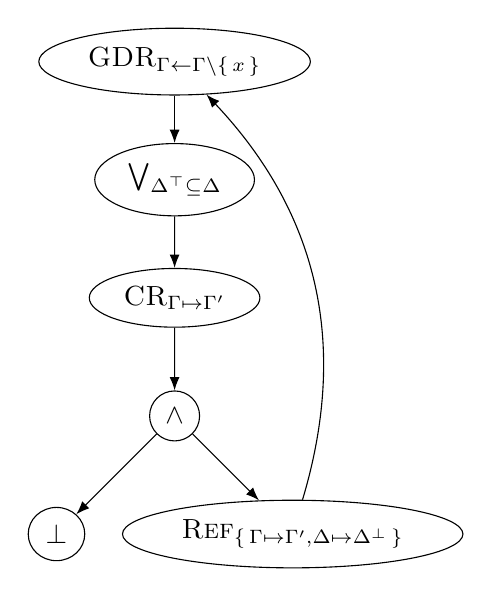
\begin{tikzpicture}[every node/.style={draw,ellipse},edge from
    parent/.style={draw,-Latex},sibling distance=3cm]
    \node (dr) {$\GDR_{\Gamma \gets \Gamma \setminus \{\, x \,\}}$}
    child {node {$\bigvee_{\Delta^\top \subseteq \Delta}$}
      child {node {$\CR_{\Gamma \mapsto \Gamma'}$}
        child {
          node[circle] {$\wedge$}
          child {node {$\bot$}}
          child {node (ref) {$\Reff_{\{\, \Gamma \mapsto \Gamma', \Delta \mapsto \Delta^{\bot} \,\}}$}}
        }}};
    \draw[-Latex, bend right] (ref) to (dr);
  \end{tikzpicture}
  \caption{A simplified version of an FCG constructed by \textsc{Crane} for the
    problem of counting partial injections from \cref{example:first}. Label
    $\bigvee_{\Delta^\top \subseteq \Delta}$ denotes set-disjunction, $\land$
    denotes conjunction, and $\bot$ denotes a contradiction---see the work by
    \citet{DBLP:conf/ijcai/BroeckTMDR11} for the descriptions of these node
    types. Here we omit some parameters as well as nodes whose only arithmetic
    effect is multiplication by one.}\label{fig:examplefcg}
\end{figure}
% Some of these nodes play an important role in the weighted version of the
% problem, whereas others are remnants of the interaction between compilation
% rules and the way in which \textsc{ForcLift} handles existential quantifiers.

% TODO: Again for the reader who is not very familiar with this area it might be
% good to at least give the circuit for one of the examples such as a
% disjunction just to show them how it is usually done.

% \footnote{Imposing an ordering on outgoing edges is just a limited version of
% edge labelling.}

% From circuits to graphs.
A \emph{first-order deterministic decomposable negation normal form
  computational graph} (FCG) is a (weakly connected) directed graph with a
single source, node labels, and ordered outgoing edges. Node
labels consist of two parts: the \emph{type} and the \emph{parameters}. The type
of a node determines its out-degree.

% TODO: I think there is a point of confusion here. Firstly the work of guy
% introduce circuits and I presume that you want to say that the node types are
% present in both the circuits as well as your structure. Given that I think you
% should start of the paragraph by saying that like with circuit introduced by
% Guy, there are node type such as XYZN. In addition to those you will be
% introducing the following new ones.
%
% I think the other point that is not made very clear is that you have no
% formally defined circuits. So perhaps if you could introduce a quick
% definition and then say that we have the same building blocks as those, ie
% nodes, but with a different graphical structure it will become clearer

Along with many node types defined previously
\citep{DBLP:conf/nips/Broeck11,DBLP:conf/ijcai/BroeckTMDR11}, \textsc{Crane}
uses three more:
\begin{itemize}
  \item a type for constraint removal denoted by $\CR$,
  \item a type for generalised domain recursion denoted by $\GDR$ (both with
        out-degree one),
  \item and $\star$---a placeholder type (with out-degree zero) for nodes that
        are going to be replaced.
\end{itemize}
Similarly to \citet{DBLP:conf/ijcai/BroeckTMDR11}, we write $T_p$ for an FCG
that has a node with the label $T_p$ (i.e., type $T$ and parameter(s) $p$) and
$\star$'s as all of its direct successors. See \cref{fig:examplefcg} for an
example FCG\@. Its source node has out-degree 1, label
$\GDR_{\Gamma \gets \Gamma \setminus \{\, x \,\}}$, and type $\GDR$.

% Connecting FCGs with formulas
Finally, we introduce a structure that represents a solution to a (W)FOMC
problem while it is still being built. A \emph{chip} is a pair $(G, L)$, where
$G$ is an FCG, and $L$ is a list of formulas, s.t. $|L|$ is equal to the number
of $\star$'s in $G$. $L$ contains formulas that still need to be compiled. Once
a formula is compiled, it replaces one of the $\star$'s in $G$ according to a
set order. We say that an FCG is \emph{complete} (i.e., it represents a
\emph{complete solution}) if it has no $\star$'s. Similarly, a chip is complete
if its FCG is complete (or, equivalently, the list of formulas is empty).

\section{New Compilation Rules}\label{sec:rules}

A \emph{(compilation) rule} takes a formula and returns a set of chips. The
cardinality of this set is the number of different ways in which the rule can be
applied to the input formula. While \textsc{ForcLift}
\citep{DBLP:conf/ijcai/BroeckTMDR11} heuristically chooses one of them, in an
attempt to not miss a solution, \textsc{Crane} returns them all. In particular,
if a rule returns an empty set, then that rule does not apply to the formula.

\subsection{Generalised Domain Recursion}\label{sec:dr}

% Main idea
The main idea behind domain recursion (both the original version by
\citet{DBLP:conf/nips/Broeck11} and the one presented here) is as follows. Let
$\Omega \in \mathcal{D}$ be a domain. Assuming that $\Omega \ne \emptyset$, pick
some $x \in \Omega$. Then, for every variable $X \in \Omega$ that occurs in a
literal, consider two possibilities: $X = x$ and $X \ne x$.

\begin{example}\label{example:dr}
  Let $\phi$ be a formula with a single clause
  \begin{multline*}
    (\{\, \neg p(X, Y), \neg p(X, Z) \,\}, \{\, (Y, Z) \,\}, \\
    \{\, X \mapsto \Gamma, Y \mapsto \Delta, Z \mapsto \Delta \,\}).
  \end{multline*}
  Then we can introduce constant $x \in \Gamma$ and rewrite $\phi$ as
  $\phi' = \{\, c_{1}, c_{2} \,\}$, where
  \begin{align*}
    c_{1} &= \begin{multlined}[t]
      (\{\, \neg p(x, Y), \neg p(x, Z) \,\}, \{\, (Y, Z) \,\}, \\
      \{\, Y \mapsto \Delta, Z \mapsto \Delta \,\}),
      \end{multlined}\\
    c_{2} &= \begin{multlined}[t]
      (\{\, \neg p(X, Y), \neg p(X, Z) \,\}, \{\, (X, x), (Y, Z) \,\}, \\
      \{\, X \mapsto \Gamma', Y \mapsto \Delta, Z \mapsto \Delta \,\}),
      \end{multlined}
  \end{align*}
    and $\Gamma' = \Gamma \setminus \{\, x \,\}$.
\end{example}

% Original domain recursion
\citet{DBLP:conf/nips/Broeck11} imposes stringent preconditions on the input
formula to ensure that the expanded version of the formula (as in
\cref{example:dr}) can be handled efficiently. For example, at least one clause
must contain a variable that occurs in all of its atoms. The clauses in this
expanded formula are then partitioned into three parts based on whether the
transformation introduced constants or constraints or both. The preconditions
ensure that these parts can be treated independently.

\begin{algorithm}[t]
  \caption{The compilation rule for $\GDR$ nodes.}\label{alg:domainrecursion}
  \KwIn{formula $\phi$, set of all relevant domains $\mathcal{D}$}
  \KwOut{set of chips $S$}
  $S \gets \emptyset$\;
  \ForEach{domain $\Omega \in \mathcal{D}$ s.t.\ there is $c \in \phi$ and $X \in \Vars(L_c)$ s.t. $\delta_c(X) = \Omega$\label{line:condition}}{
    $\phi' \gets \emptyset$\;
    $x \gets \text{a new constant in domain } \Omega$\;
    \ForEach{clause $c = (L, C, \delta) \in \phi$\label{line:forclause}}{
      $V \gets \{\, X \in \Vars(L) \mid \delta(X) = \Omega \,\}$\;
      \ForEach{subset $W \subseteq V$ s.t. $W^2 \cap C = \emptyset$ {\bf and} $W \cap \{\, X \in \Vars(C) \mid (X, y) \in C \text{ for some constant } y \,\} = \emptyset$\label{line:conditions}}{
        \tcc{$\delta'$ restricts $\delta$ to the new set of variables}
        $\phi' \gets \phi' \cup \{\, (L[x/W], C[x/W] \cup \{\, (X, x) \mid (X \in V \setminus W) \,\}, \delta') \,\}$\;\label{line:generation}
      }
    }
    $S \gets S \cup \{\, (\GDR_{\Omega \gets \Omega \setminus \{\, x \,\}}, \langle\phi'\rangle) \,\}$\;
  }
\end{algorithm}

% Description of GDR, in contrast to DR
In contrast, GDR has only one precondition: for GDR to be applicable on domain
$\Omega \in \mathcal{D}$, there must be at least one variable with domain
$\Omega$ that is featured in a literal (and not just in constraints). Without
such variables, GDR would have no effect on the formula. GDR is also simpler in
that the expanded formula is left as-is to be handled by other compilation
rules. Typically, after a few more rules are applied, a combination of $\CR$ and
$\Reff$ nodes introduces a cycle-inducing edge back to the $\GDR$ node, thus
completing the definition of a recursive function. The GDR compilation rule is
summarised as \cref{alg:domainrecursion} and explained in more detail using the
example below.

\begin{example}
  Let $\phi \coloneqq \{\, c_1, c_2 \,\}$ be the formula from
  \cref{example:first}. While GDR is possible on both domains, here we
  illustrate how it works on $\Gamma$. Having chosen a domain, the algorithm
  iterates over the clauses of $\phi$. Suppose \cref{line:forclause} picks
  $c = c_1$ as the first clause. Then, set $V$ is constructed to contain all
  variables with domain $\Omega = \Gamma$ that occur in the literals of clause
  $c$. In this case, $V = \{\, X \,\}$.

  \Cref{line:conditions} iterates over all subsets $W \subseteq V$ of variables
  that can be replaced by a constant without resulting in evidently
  unsatisfiable formulas. We impose two restrictions on $W$. First,
  $W^2 \cap C = \emptyset$ ensures that there are no pairs of variables in $W$
  that are constrained to be distinct, since that would result in an $x \ne x$
  constraint after substitution. Similarly, we want to avoid variables in $W$
  that have inequality constraints with constants: after the substitution, such
  constraints would transform into inequality constraints between two constants.
  In this case, both subsets of $V$ satisfy these conditions, and
  \cref{line:generation} generates two clauses for the output formula:
  \begin{multline*}
    (\{\, \neg p(X, Y), \neg p(X, Z) \,\}, \{\, (Y, Z), (X, x) \,\}, \\
    \{\, X \mapsto \Gamma, Y \mapsto \Delta, Z \mapsto \Delta \,\}),
  \end{multline*}
  from $W = \emptyset$ and
  \[
    (\{\, \neg p(x, Y), \neg p(x, Z) \,\}, \{\, (Y, Z) \,\}, \{\, Y \mapsto \Delta, Z \mapsto \Delta \,\})
  \]
  from $W = V$.

  When \cref{line:forclause} picks $c = c_2$, then $V = \{\, X, Z \,\}$. The
  subset $W = V$ fails to satisfy the conditions on \cref{line:conditions}
  because of the $X \ne Z$ constraint. The other three subsets of $V$ all
  generate clauses for $\phi'$. Indeed, $W = \emptyset$ generates
  \begin{multline*}
    (\{\, \neg p(X, Y), \neg p(Z, Y) \,\}, \{\, (X, Z), (X, x), (Z, x) \,\}, \\
    \{\, X \mapsto \Gamma, Y \mapsto \Delta, Z \mapsto \Gamma \,\}),
  \end{multline*}
  $W = \{\, X \,\}$ generates
  \[
    (\{\, \neg p(x, Y), \neg p(Z, Y) \,\}, \{\, (Z, x) \,\}, \{\, Y \mapsto \Delta, Z \mapsto \Gamma \,\}),
  \]
  and $W = \{\, Z \,\}$ generates
  \[
    (\{\, \neg p(X, Y), \neg p(x, Y) \,\}, \{\, (X, x) \,\}, \{\, X \mapsto \Gamma, Y \mapsto \Delta \,\}).
  \]
\end{example}

\subsection{Constraint Removal}\label{sec:cr}

\begin{algorithm}[t]
  \caption{The compilation rule for $\CR$ nodes.}\label{alg:constraintremoval}
  \KwIn{formula $\phi$, set of all relevant domains $\mathcal{D}$}
  \KwOut{set of chips $S$}
  $S \gets \emptyset$\;
  \ForEach{domain $\Omega \in \mathcal{D}$ and element $x \in \Omega$ s.t. $x$ does not occur in any literal of any clause of $\phi$ {\bf and} for each clause $c = (L, C, \delta_c) \in \phi$ and variable $X \in \Vars(c)$, either $\delta_c(X) \ne \Omega$ or $(X, x) \in C$\label{line:crconditions}}{
    add a new domain $\Omega'$ to $\mathcal{D}$\;
    $\phi' \gets \emptyset$\;
    \ForEach{clause $(L, C, \delta) \in \phi$}{
      $C' \gets \{\, (a, b) \in C \mid b \ne x \,\}$\;\label{line:constraintremoval}
      \nosemic$\delta' \gets X \mapsto
      \begin{cases}
        \Omega' & \text{if } \delta(X) = \Omega\\
        \delta(X) & \text{otherwise;}
      \end{cases}$\;\label{line:newdelta}
      $\phi' \gets \phi' \cup \{\, (L, C', \delta') \,\}$\;
    }
    $S \gets S \cup \{\, (\CR_{\Omega \mapsto \Omega'}, \langle\phi'\rangle) \,\}$\;
  }
\end{algorithm}

Recall that GDR on a domain $\Omega$ creates constraints of the form $X_i \ne x$
for some constant $x \in \Omega$ and family of variables $X_i \in \Omega$. Once
certain conditions are satisfied, \cref{alg:constraintremoval} can eliminate
these constraints and replace $\Omega$ with a new domain $\Omega'$, which can be
interpreted as $\Omega \setminus \{\, x \,\}$. These conditions (on
\cref{line:crconditions} of the algorithm) are that a constraint of the form
$X \ne x$ exists for all variables $X \in \Omega$ across all clauses, and such
constraints are the only place where $x$ occurs. The algorithm then proceeds to
construct the new formula by removing constraints (on
\cref{line:constraintremoval}) and constructing a new domain map $\delta'$ that
replaces $\Omega$ with $\Omega'$ (on \cref{line:newdelta}).

\begin{example}
  Let $\phi = \{\, c_1, c_2 \,\}$ be a formula with clauses
  \begin{align*}
    c_1 &=
          \begin{multlined}[t]
            (\{\, \neg p(X, Y), \neg p(X, Z) \,\}, \{\, (X, x), (Y, Z) \,\}, \\
            \{\, X \mapsto \Gamma, Y \mapsto \Delta, Z \mapsto \Delta \,\}),
          \end{multlined}\\
    c_2 &=
          \begin{multlined}[t]
            (\{\, \neg p(X, Y), \neg p(Z, Y) \,\}, \\
            \{\, (X, x), (Z, X), (Z, x) \,\}, \\
            \{\, X \mapsto \Gamma, Y \mapsto \Delta, Z \mapsto \Gamma \,\}).
          \end{multlined}
  \end{align*}
  Domain $\Gamma$ and its element $x \in \Gamma$ satisfy the preconditions for
  CR\@. The rule introduces a new domain $\Gamma'$ and transforms $\phi$ to
  $\phi' = (c_1', c_2')$, where
  \begin{align*}
    c_1' &=
           \begin{multlined}[t]
             (\{\, \neg p(X, Y), \neg p(X, Z) \,\}, \{\, (Y, Z) \,\}, \\
             \{\, X \mapsto \Gamma', Y \mapsto \Delta, Z \mapsto \Delta \,\}),
           \end{multlined} \\
    c_2' &=
           \begin{multlined}[t]
             (\{\, \neg p(X, Y), \neg p(Z, Y) \,\}, \{\, (Z, X) \,\}, \\
             \{\, X \mapsto \Gamma', Y \mapsto \Delta, Z \mapsto \Gamma' \,\}).
           \end{multlined}
  \end{align*}
\end{example}

\subsection{Identifying Opportunities for Recursion}\label{sec:ref}

\paragraph{Notation.}
Let $\Doms$ be a function that maps any clause or formula to the set of domains
used within, and let $\dom(f)$ denote the domain of function $f$.

\paragraph{Hashing.}
We use (integer-valued) hash functions to discard pairs of formulas that are too
different for recursion to work. The hash code of a clause
$c = (L, C, \delta_{c})$ (denoted by $\# c$) combines the hash codes of the sets
of constants and predicates in $c$, the numbers of positive and negative
literals, the number of inequality constraints $|C|$, and the number of
variables $|\Vars(c)|$. The hash code of a formula $\phi$ combines the hash
codes of all its clauses and is denoted by $\#\phi$.

\paragraph{Caching.}
\textsc{ForcLift} \citep{DBLP:conf/ijcai/BroeckTMDR11} uses a cache to check if
a formula is identical to one of the formulas that have already been fully
compiled. To facilitate recursion, we extend the caching scheme to include
formulas that have been encountered but not fully compiled yet. Formally, we
define a \emph{cache} to be a map from integers (e.g., hash codes) to sets of
pairs of the form $(\phi, v)$, where $\phi$ is a formula, and $v$ is an FCG
node.

\begin{algorithm}[t]
  \caption{The compilation rule for $\Reff$ nodes.}\label{alg:trycache}
  \KwIn{formula $\phi$, cache $C$}
  \KwOut{a set of chips}

  \ForEach{formula and node $(\psi, v) \in C(\#\phi)$}{
    $\rho \gets \identifyRecursion{$\phi$, $\psi$}$\;
    \lIf{$\rho \ne {\normalfont \texttt{null}}$}{\Return{$\{\, (\Reff_\rho(v), \langle\rangle) \,\}$}}
  }
  \Return{$\emptyset$}\;

  \Fn{\identifyRecursion{formula $\phi$, formula $\psi$, map $\rho = \emptyset$}}{
    \lIf{$|\phi| \ne |\psi|$ {\bf or} $\#\phi \ne \#\psi$}{\Return{\normalfont\texttt{null}}}
    \lIf{$\phi = \emptyset$}{\Return{$\rho$}}
    \ForEach{clause $c \in \psi$\label{line:for1}}{
      \ForEach{clause $d \in \phi$ s.t. $\#d=\#c$\label{line:for2}}{
        \ForAll{$\gamma \in \generateMaps{$c$, $d$, $\rho$}$\label{line:generateMaps}}{
          $\rho' \gets \identifyRecursion{$\phi\setminus\{\, d \,\}$, $\psi\setminus\{\, c \,\}$, $\rho\cup\gamma$}$\;\label{line:recursion}
          \lIf{$\rho' \ne {\normalfont \texttt{null}}$}{\Return{$\rho'$}}
        }
      }
      \Return{\normalfont\texttt{null}}\;
    }
  }
\end{algorithm}

% Cache $C$ is used to partition all previously-encountered formulas based on
% their hash codes.
\Cref{alg:trycache} describes the compilation rule for creating $\Reff$ nodes.
For every formula $\psi$ in the cache s.t. $\#\psi = \#\phi$, function
\texttt{r} is called to check whether a recursive call is feasible. If it is,
\texttt{r} returns a (total) map $\rho\colon \Doms(\psi) \to \Doms(\phi)$ that
shows how $\psi$ can be transformed into $\phi$ by replacing each domain
$\Omega \in \Doms(\psi)$ with $\rho(\Omega) \in \Doms(\phi)$. Otherwise,
\texttt{r} returns \texttt{null} to signify that $\phi$ and $\psi$ are too
different for recursion to work. This happens if $\phi$ and $\psi$ (or their
subformulas explored in recursive calls) are structurally different (i.e., the
numbers of clauses or the hash codes fail to match) or if a clause of $\psi$
cannot be paired with a sufficiently similar clause of $\phi$. Function
\texttt{r} works by iterating over pairs of clauses of $\phi$ and $\psi$ that
have the same hash codes. For every pair of sufficiently similar clauses,
\texttt{r} calls itself on the remaining clauses until the map
$\rho\colon \Doms(\psi) \pfun \Doms(\phi)$ becomes total, and all clauses are
successfully coupled.

Function \texttt{genMaps} checks the compatibility of a pair of clauses. It
considers every possible bijection $\beta\colon \Vars(c) \to \Vars(d)$ and map
$\gamma\colon \Doms(c) \to \Doms(d)$ s.t.
\[
  \begin{tikzcd}
    \Vars(c) \ar[r, dashed, "\beta"] \arrow[d, swap, "\delta_c"] & \Vars(d) \ar[d, "\delta_d"] \\
    \Doms(c) \ar[r, dashed, "\gamma"] \ar[d, hookrightarrow] & \Doms(d) \ar[d, hookrightarrow] \\
    \Doms(\psi) \ar[r, swap, "\rho", "|" marking, outer sep=5pt] & \Doms(\phi).
  \end{tikzcd}
\]
commutes, and $c$ becomes equal to $d$ when its variables are replaced according
to $\beta$ and its domains replaced according to $\gamma$. The function then
returns each such $\gamma$ as soon as possible. The commutativity check also
ensures that $\rho \cup \gamma$ is possible on \cref{line:recursion} of
\cref{alg:trycache}. The resulting (partial) function $\rho \cup \gamma$ is the
unique function s.t. $\rho \cup \gamma|_{\dom(\rho)} = \rho$, and
$\rho \cup \gamma|_{\dom(\gamma)} = \gamma$. The operation is defined when
$\rho|_{\dom(\rho)\cap\dom(\gamma)} = \gamma|_{\dom(\rho)\cap\dom(\gamma)}$.

\section{How to Interpret an FCG}\label{sec:interpret}

When \textsc{ForcLift} \citep{DBLP:conf/ijcai/BroeckTMDR11} compiles a WFOMC
instance into a circuit, each node type encodes an arithmetic operation on its
inputs and parameters. These operations are then immediately performed while
traversing the circuit. With \textsc{Crane}, the interpretation of an FCG is a
collection of functions. Each function has (some) domain sizes as parameters and
may contain recursive calls to other functions, including itself. While there
may be any number of subsidiary functions, there is always one main function
that can be called with the sizes of the domains of the input formula as
arguments. Henceforth, this function is always called $f$, and it is defined by
the source node.

The interpretation of a node is decided by its type. Here we describe the
interpretations of new (or significantly changed) types and refer the reader to
previous work \citep{DBLP:conf/ijcai/BroeckTMDR11} for information on other
types. The interpretation of a $\CR$ or a $\GDR$ node is simply the
interpretation of its only direct successor. Obviously, $\star$ nodes have no
interpretation as incomplete FCGs are not meant to be interpreted. The
interpretation of a $\Reff$ node is a function call. The direct successor of the
$\Reff$ node (say, $v$) then must introduce a function. The parameters of this
function are the sizes of all domains used by nodes reachable from $v$.

\begin{example}\label{example:interpretation}
  Consider the FCG from \cref{fig:examplefcg}. The input formula (i.e., the
  formula from \cref{example:first}) has two domains: $\Gamma$ and $\Delta$.
  Thus, the interpretation of the FCG is a function
  $f\colon \mathbb{N}_{0} \times \mathbb{N}_{0} \to \mathbb{R}_{\ge 0}$. Let
  $m \coloneqq |\Gamma|$, and $n \coloneqq |\Delta|$. The node labelled
  $\bigvee_{\Delta^{\top} \subseteq \Delta}$ tells us that
  $f(m, n) = \sum_{l = 0}^{n} \binom{n}{l} \square$, where $\square$ is the
  interpretation of the remaining subgraph, and $l$ iterates over all possible
  sizes of $\Delta^{\top}$. It also creates two subdomains
  $\Delta^{\top}, \Delta^{\bot} \subseteq \Delta$ that partition $\Delta$, i.e.,
  as the size of $\Delta^{\top}$ increases, the size of $\Delta^{\bot}$
  correspondingly decreases. Nodes labelled $\land$ correspond to
  multiplication. Therefore,
  $f(m, n) = \sum_{l = 0}^{n} \binom{n}{l} \diamondsuit \times \heartsuit$,
  where $\diamondsuit$ is the interpretation of the contradiction (i.e., $\bot$)
  node, and $\heartsuit$ is the interpretation of the $\Reff$ node.

  A contradiction node with clause $c$ as a parameter is interpreted as one if
  the clause has groundings and zero otherwise. In this case, the parameter is
  $c = (\emptyset, \{\, (X, Y) \,\}, \{\, X \mapsto \Delta^\top, Y \mapsto \Delta^\top \,\})$
  (not shown in \cref{fig:examplefcg}), which can be read as
  $\forall X, Y \in \Delta^{\top}\text{. }X \ne Y \implies \bot$, i.e.,
  $\forall X, Y \in \Delta^{\top}\text{. }X = Y$. This latter sentence is true
  if and only if $|\Delta^{\top}| < 2$. Therefore, we can use the Iverson
  bracket notation to write
  \[
    \diamondsuit = [l < 2] \coloneqq
    \begin{cases}
      1 & \text{if } l < 2 \\
      0 & \text{otherwise.}
    \end{cases}
  \]

  It remains to interpret the $\Reff$ node. Parameter
  $\{\, \Gamma \mapsto \Gamma', \Delta \mapsto \Delta^\bot \,\}$ tells us that
  the interpretation of the $\Reff$ node should be the same as that of the
  source node, but with domains $\Gamma$ and $\Delta$ replaced with $\Gamma'$
  and $\Delta^{\bot}$, respectively. Domain $\Gamma'$ was created by the CR rule
  applied on $\Gamma$, so $|\Gamma'| = m - 1$. Now
  $\Delta^{\bot} = \Delta \setminus \Delta^{\top}$, and $|\Delta^{\top}| = l$,
  so $|\Delta^{\bot}| = n - l$. Thus, the interpretation of the $\Reff$ node is
  a recursive call to $f(m - 1, n - l)$. Therefore,
  \begin{align}
    f(m, n) &= \sum_{l = 0}^{n} \binom{n}{l} [l < 2] f(m-1, n-l)\nonumber \\
            &= f(m-1, n) + n f(m-1, n-1).\label{eq:solution}
  \end{align}
  To use this recursive function to compute the model count of the input formula
  for any domain sizes, one just needs to find the base cases $f(0, n)$ and
  $f(m, 0)$ for all $m, n \in \mathbb{N}_{0}$.
\end{example}

\section{Empirical Results}\label{sec:results} % Newly Domain-Liftable Formulas

\begin{table*}[t]
  \centering
  \begin{tabular}{cccccc}
    \toprule
    \multicolumn{3}{c}{Function Class} & \multicolumn{3}{c}{Asymptotic Complexity of Counting} \\
    Partial & Endo- & Class & Best Known & With \textsc{ForcLift} & With \textsc{Crane} \\
    \midrule
    \rowcolor{gray!10}\cmark/\xmark & \cmark/\xmark & Functions & $\log m$ & $m$ & $m$ \\
    \xmark & \xmark & \multirow{4}{*}{Surjections} & $n \log m$ & $m^{3}+n^{3}$ & $m^{3}+n^{3}$ \\
    \xmark & \cmark & & $m \log m$ & $m^{3}$ & $m^{3}$ \\
    \cmark & \xmark & & \multicolumn{3}{c}{Same as injections from $\Delta$ to $\Gamma$} \\
    \cmark & \cmark & & \multicolumn{3}{c}{Same as endo-injections} \\
    \rowcolor{gray!10}\xmark & \xmark & & $m$ & --- & $mn$ \\
    \rowcolor{gray!10}\xmark & \cmark & & $m$ & --- & $m^3$ \\
    \rowcolor{gray!10}\cmark & \xmark & & $\min\{\, m, n \,\}^2$ & --- & $mn$ \\
    \rowcolor{gray!10}\cmark & \cmark & \multirow{-4}{*}{Injections} & $m^2$ & --- & --- \\
    \xmark & \xmark & \multirow{3}{*}{Bijections} & $m$ & --- & $m$ \\
    \xmark & \cmark & & \multicolumn{3}{c}{\multirow{2}{*}{Same as (partial) (endo-)injections}} \\
    \cmark & \cmark/\xmark & & \multicolumn{3}{c}{} \\
    \bottomrule
  \end{tabular}
  \caption{The worst-case complexity of counting various types of functions.
    Here, $m$ is the size of domain $\Gamma$, and $n$ is the size of domain
    $\Delta$. All asymptotic complexities are in $\Theta(\cdot)$. A dash means
    that no complete solution was found.}\label{tbl:results}
\end{table*}
% TODO: It is a standard to discuss a few lifted theories like the smokers and
% friends example. Can you also include some empirical results on such theories
% as well to appeal to the sanity of the reader that it actually works for
% problems in frameworks such as Markov log networks

We compare \textsc{Crane} and \textsc{ForcLift}
\citep{DBLP:conf/ijcai/BroeckTMDR11} on their ability to count various kinds of
functions. This class of instances is chosen because of its simplicity and
ubiquity and the inability of state-of-the-art WFOMC algorithms to solve many
such instances. Note that other WFOMC algorithms---\textsc{L2C}
\citep{DBLP:conf/kr/KazemiP16} and probabilistic theorem proving
\citep{DBLP:journals/cacm/GogateD16}---are unable to solve any of the instances
that \textsc{ForcLift} fails on. We begin by describing how such
function-counting problems can be expressed in FOL\@. \textsc{ForcLift} then
translates these sentences in FOL to formulas as defined in \cref{def:formula}.

% Describe what kind of instances we're investigating
Let $p \in \Gamma \times \Delta$ be a predicate. To restrict all relations
representable by $p$ to just functions from $\Gamma$ to $\Delta$, in FOL one
might write
\[
  \forall X \in \Gamma\text{. }\forall Y, Z \in \Delta\text{. }p(X, Y) \land p(X, Z) \implies Y = Z
\]
and
\begin{equation}\label{eq:def2}
  \forall X \in \Gamma\text{. }\exists Y \in \Delta\text{. }p(X, Y).
\end{equation}
The former sentence says that one element of $\Gamma$ can map to at \emph{most}
one element of $\Delta$, and the latter sentence says that each element of
$\Gamma$ must map to at \emph{least} one element of $\Delta$. One can then add
\[
  \forall X,Z \in \Gamma\text{. }\forall Y \in \Delta\text{. }p(X, Y) \land p(Z, Y) \implies X = Z
\]
to restrict $p$ to injections or
\[
  \forall Y \in \Delta\text{. }\exists X \in \Gamma\text{. }p(X, Y)
\]
to ensure surjectivity or remove \cref{eq:def2} to consider partial functions.
Lastly, one can replace all occurrences of $\Delta$ with $\Gamma$ to model
endofunctions (i.e., functions with the same domain and codomain) instead.

In our experiments, we consider all sixteen combinations of these properties,
i.e., injectivity, surjectivity, partiality, and endo-. \textsc{ForcLift} is
always run until it terminates. \textsc{Crane} is run until either five
solutions are found or the search tree reaches height 6 (which happens in at
most a few seconds). If successful, \textsc{ForcLift} generates a circuit, and
\textsc{Crane} generates one or more (complete) FCGs. In both cases, we manually
convert the resulting graphs into definitions of functions as described in
\cref{sec:interpret}. We then assess the complexity of each solution and pick
the best if \textsc{Crane} returns several solutions of varying complexities.
When assessing the complexity of each such definition, we make two assumptions.
First, we can compute the binomial coefficient $\binom{n}{k}$ in $\Theta(nk)$
time. Second, techniques such as dynamic programming and memoization are used to
avoid recomputing the same binomial coefficient or function call multiple times.

The experimental results are in \cref{tbl:results}. Previous work often compares
WFOMC algorithms by running them on a few instances with increasing domain sizes
and measuring runtime
\citep{DBLP:conf/nips/Broeck11,DBLP:conf/ijcai/BroeckTMDR11,DBLP:conf/aaai/BroeckD12}.
However, we can do better than that and identify the exact worst-case asymptotic
complexity of a solution produced by either \textsc{Crane} or \textsc{ForcLift}.
The best-known asymptotic complexity for computing total surjections is by
\citet{30049}. All other best-known complexity results are inferred from the
formulas and programs on the on-line encyclopedia of integer sequences
\citep{oeis}. On instances that could already be solved by \textsc{ForcLift},
the two algorithms perform equally well. However, \textsc{Crane} can also solve
all but one instances that \textsc{ForcLift} fails on in at most cubic time.

Let us examine the case of counting partial (non-endomorphic) injections more
closely. The FCG in \cref{fig:examplefcg,example:interpretation} counts partial
injections and is responsible for the $mn$ entry in the table. For a complete
solution, \cref{eq:solution} must be combined with the base case $f(0, n) = 1$
for all $n \in \mathbb{N}_{0}$. This base case says that the empty partial map
is the only partial injection with an empty domain. Finally, note that $f(m, n)$
can be evaluated in $\Theta(mn)$ time by a dynamic programming algorithm that
computes $f(i, j)$ for all $i = 0, \dots, m$ and $j = 0, \dots, n$.

\section{Conclusion and Future Work}\label{sec:conclusion}

% A summary of what's been done/achieved and how

In this paper, we showed how a state-of-the-art (W)FOMC algorithm can be
empowered by generalising domain recursion and adding support for cycles in the
graph that encodes a solution. To construct such graphs, \textsc{Crane}
supplements \textsc{ForcLift} \citep{DBLP:conf/ijcai/BroeckTMDR11} with three
new compilation rules. Our experiments revealed a range of counting problems
that are liftable to \textsc{Crane} but not to any other (W)FOMC algorithm.
Although in this paper we focus on unweighted counting, \textsc{ForcLift}'s
support for weights trivially transfers to \textsc{Crane} as well. The common
thread across these newly liftable problems is (partial) injectivity. Thus, we
can formulate the following conjecture.

\begin{conjecture}
  Let \IFO{} be the class of formulas in FOL that contain clauses with at most
  two variables as well as any number of copies of
  \begin{align*}
    &\begin{multlined}[t]
      (\forall X \in \Gamma\text{. }\forall Y, Z \in \Delta\text{. }\\
      Y \ne Z \implies \neg p(X, Y) \lor \neg p(X, Z)) \land
    \end{multlined}\\
    &\begin{multlined}[t]
      (\forall X, Z \in \Gamma\text{. }\forall Y \in \Delta\text{. }\\
      X \ne Z \implies \neg p(X, Y) \lor \neg p(Z, Y))
    \end{multlined}
  \end{align*}
  for some predicate $p$ and domains $\Gamma$ and $\Delta$. Then \IFO{} is
  liftable by \textsc{Crane}.
\end{conjecture}

Recall that \Ctwo{} is the class of formulas with counting quantifiers and at
most two variables. \Ctwo{} was recently shown to be liftable
\citep{DBLP:journals/jair/Kuzelka21} but without providing a usable (W)FOMC
algorithm. Since the tasks of counting injections and bijections fall into the
\Ctwo{} fragment, we can conjecture the following.

\begin{conjecture}
  \Ctwo{} is liftable by \textsc{Crane} by either reformulating formulas in
  \Ctwo{} to avoid counting quantifiers or extending \textsc{Crane} to support
  them.
\end{conjecture}

However, the most important direction for future work is to fully automate this
new process. First, we need an algorithm that transforms FCGs into definitions
of functions. Formalising this process would also allow us to prove the
correctness of the new compilation rules in constructing FCGs that indeed
compute the right (weighted) model counts. Second, these definitions must be
simplified before they can be used, perhaps by a computer algebra system. Third,
we need a way to find the base cases for the recursive definitions provided by
\textsc{Crane}. Fourth, since the first solution found by \textsc{Crane} is not
always optimal in terms of its complexity, an automated way to determine the
asymptotic complexity of a solution would be helpful as well. Achieving these
goals would enable \textsc{Crane} to automatically constructing efficient ways
to compute various functions and sequences. In addition to the potential impact
on areas of artificial intelligence (AI) such as statistical relational AI
\citep{DBLP:series/synthesis/2016Raedt}, \textsc{Crane} could be beneficial to
research in combinatorics as well \citep{DBLP:conf/ilp/BarvinekB0ZK21}.

\bibliography{paper}
\end{document}
